\definecolor{myblue}{RGB}{166, 189, 219}
\definecolor{mygray}{RGB}{211, 211, 211}
\definecolor{mypink}{RGB}{255, 166, 201}
% \definecolor{bgun}{RGB}{203, 101, 96} % B-GUN color

% \definecolor{darkslategray38}{RGB}{38,38,38}
\definecolor{indianred19364103}{RGB}{193,64,103}
% \definecolor{lightgray204}{RGB}{204,204,204}
\definecolor{steelblue51132141}{RGB}{51,132,141}
\definecolor{stackconv}{RGB}{240, 160, 75}
\definecolor{myred}{RGB}{255, 138, 138}

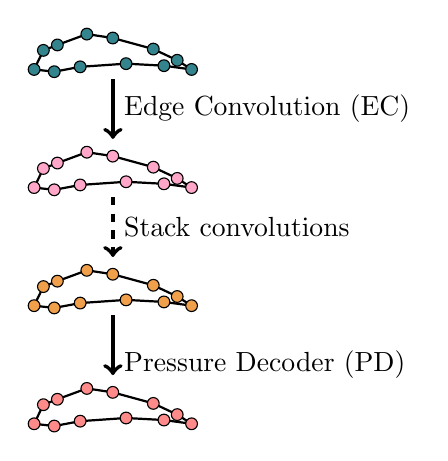
\begin{tikzpicture}[scale=1, 
                    nodeout/.style={rectangle, fill=mypink, opacity=1, minimum width=2.5mm, minimum height=2.5mm, inner sep=0pt, line width=0.5pt, draw=black}, nodehidden/.style={circle, fill=mygray, opacity=1, minimum size=2.5mm, inner sep=0pt, line width=0.5pt, draw=black}, 
                    nodein/.style={rectangle, fill=myblue, minimum width=2mm, minimum height=2mm, inner sep=0pt, line width=0.5pt, draw=black}]

    \def\scaleFactor{2} % Define scaling factor
    \def\circleDia{1.5}
    % Define the points for the input airfoil shape with scaling
    \coordinate (P0) at ({\scaleFactor * 0.9996}, {\scaleFactor * 0.0008});
    \coordinate (P1) at ({\scaleFactor * 0.9083}, {\scaleFactor * 0.0590});
    \coordinate (P2) at ({\scaleFactor * 0.7565}, {\scaleFactor * 0.1303});
    \coordinate (P3) at ({\scaleFactor * 0.4992}, {\scaleFactor * 0.2004});
    \coordinate (P4) at ({\scaleFactor * 0.3345}, {\scaleFactor * 0.2253});
    \coordinate (P5) at ({\scaleFactor * 0.1474}, {\scaleFactor * 0.1564});
    \coordinate (P6) at ({\scaleFactor * 0.0586}, {\scaleFactor * 0.1220});
    \coordinate (P7) at ({\scaleFactor * -0.0004}, {\scaleFactor * 0.0008});
    \coordinate (P8) at ({\scaleFactor * 0.1276}, {\scaleFactor * -0.0135});
    \coordinate (P9) at ({\scaleFactor * 0.2922}, {\scaleFactor * 0.0174});
    \coordinate (P10) at ({\scaleFactor * 0.5837}, {\scaleFactor * 0.0376});
    \coordinate (P11) at ({\scaleFactor * 0.8242}, {\scaleFactor * 0.0246});
    \coordinate (P12) at ({\scaleFactor * 0.9996}, {\scaleFactor * 0.0008});
    
    % Draw the airfoil shape
    \draw[thick] (P0) -- (P1) -- (P2) -- (P3) -- (P4) -- (P5) -- (P6) -- (P7) -- (P8) -- (P9) -- (P10) -- (P11) -- (P12) -- cycle;
    
    % Add circles at selected points
    \foreach \i in {1, 2, 3, 4, 5, 6, 7, 8, 9, 10, 11, 12} {
        \node[circle, draw, fill=steelblue51132141, inner sep=\circleDia pt] at (P\i) {};
    }
    
    % Define the points for the edge conv airfoil shape
    % Define the shift in abscissa
    \def\yShift{-1.5}

    \coordinate (P0) at ({\scaleFactor * 0.9996}, {\yShift + \scaleFactor * 0.0008});
    \coordinate (P1) at ({\scaleFactor * 0.9083}, {\yShift + \scaleFactor * 0.0590});
    \coordinate (P2) at ({\scaleFactor * 0.7565}, {\yShift + \scaleFactor * 0.1303});
    \coordinate (P3) at ({\scaleFactor * 0.4992}, {\yShift + \scaleFactor * 0.2004});
    \coordinate (P4) at ({\scaleFactor * 0.3345}, {\yShift + \scaleFactor * 0.2253});
    \coordinate (P5) at ({\scaleFactor * 0.1474}, {\yShift + \scaleFactor * 0.1564});
    \coordinate (P6) at ({\scaleFactor * 0.0586}, {\yShift + \scaleFactor * 0.1220});
    \coordinate (P7) at ({\scaleFactor * -0.0004}, {\yShift + \scaleFactor * 0.0008});
    \coordinate (P8) at ({\scaleFactor * 0.1276}, {\yShift + \scaleFactor * -0.0135});
    \coordinate (P9) at ({\scaleFactor * 0.2922}, {\yShift + \scaleFactor * 0.0174});
    \coordinate (P10) at ({\scaleFactor * 0.5837}, {\yShift + \scaleFactor * 0.0376});
    \coordinate (P11) at ({\scaleFactor * 0.8242}, {\yShift + \scaleFactor * 0.0246});
    \coordinate (P12) at ({\scaleFactor * 0.9996}, {\yShift + \scaleFactor * 0.0008});
    
    % Draw the airfoil shape
    \draw[thick] (P0) -- (P1) -- (P2) -- (P3) -- (P4) -- (P5) -- (P6) -- (P7) -- (P8) -- (P9) -- (P10) -- (P11) -- (P12) -- cycle;
    
    % Add circles at selected points
    \foreach \i in {1, 2, 3, 4, 5, 6, 7, 8, 9, 10, 11, 12} {
        \node[circle, draw, fill=mypink, inner sep=\circleDia pt] at (P\i) {};
    }

    % Define the points for the stack conv airfoil shape
    % Define the shift in abscissa
    \def\yShift{-3}

    \coordinate (P0) at ({\scaleFactor * 0.9996}, {\yShift + \scaleFactor * 0.0008});
    \coordinate (P1) at ({\scaleFactor * 0.9083}, {\yShift + \scaleFactor * 0.0590});
    \coordinate (P2) at ({\scaleFactor * 0.7565}, {\yShift + \scaleFactor * 0.1303});
    \coordinate (P3) at ({\scaleFactor * 0.4992}, {\yShift + \scaleFactor * 0.2004});
    \coordinate (P4) at ({\scaleFactor * 0.3345}, {\yShift + \scaleFactor * 0.2253});
    \coordinate (P5) at ({\scaleFactor * 0.1474}, {\yShift + \scaleFactor * 0.1564});
    \coordinate (P6) at ({\scaleFactor * 0.0586}, {\yShift + \scaleFactor * 0.1220});
    \coordinate (P7) at ({\scaleFactor * -0.0004}, {\yShift + \scaleFactor * 0.0008});
    \coordinate (P8) at ({\scaleFactor * 0.1276}, {\yShift + \scaleFactor * -0.0135});
    \coordinate (P9) at ({\scaleFactor * 0.2922}, {\yShift + \scaleFactor * 0.0174});
    \coordinate (P10) at ({\scaleFactor * 0.5837}, {\yShift + \scaleFactor * 0.0376});
    \coordinate (P11) at ({\scaleFactor * 0.8242}, {\yShift + \scaleFactor * 0.0246});
    \coordinate (P12) at ({\scaleFactor * 0.9996}, {\yShift + \scaleFactor * 0.0008});
    
    % Draw the airfoil shape
    \draw[thick] (P0) -- (P1) -- (P2) -- (P3) -- (P4) -- (P5) -- (P6) -- (P7) -- (P8) -- (P9) -- (P10) -- (P11) -- (P12) -- cycle;
    
    % Add circles at selected points
    \foreach \i in {1, 2, 3, 4, 5, 6, 7, 8, 9, 10, 11, 12} {
        \node[circle, draw, fill=stackconv, inner sep=\circleDia pt] at (P\i) {};
    }

    % Define the points for the output airfoil shape
    % Define the shift in abscissa
    \def\yShift{-4.5}

    \coordinate (P0) at ({\scaleFactor * 0.9996}, {\yShift + \scaleFactor * 0.0008});
    \coordinate (P1) at ({\scaleFactor * 0.9083}, {\yShift + \scaleFactor * 0.0590});
    \coordinate (P2) at ({\scaleFactor * 0.7565}, {\yShift + \scaleFactor * 0.1303});
    \coordinate (P3) at ({\scaleFactor * 0.4992}, {\yShift + \scaleFactor * 0.2004});
    \coordinate (P4) at ({\scaleFactor * 0.3345}, {\yShift + \scaleFactor * 0.2253});
    \coordinate (P5) at ({\scaleFactor * 0.1474}, {\yShift + \scaleFactor * 0.1564});
    \coordinate (P6) at ({\scaleFactor * 0.0586}, {\yShift + \scaleFactor * 0.1220});
    \coordinate (P7) at ({\scaleFactor * -0.0004}, {\yShift + \scaleFactor * 0.0008});
    \coordinate (P8) at ({\scaleFactor * 0.1276}, {\yShift + \scaleFactor * -0.0135});
    \coordinate (P9) at ({\scaleFactor * 0.2922}, {\yShift + \scaleFactor * 0.0174});
    \coordinate (P10) at ({\scaleFactor * 0.5837}, {\yShift + \scaleFactor * 0.0376});
    \coordinate (P11) at ({\scaleFactor * 0.8242}, {\yShift + \scaleFactor * 0.0246});
    \coordinate (P12) at ({\scaleFactor * 0.9996}, {\yShift + \scaleFactor * 0.0008});
    
    % Draw the airfoil shape
    \draw[thick] (P0) -- (P1) -- (P2) -- (P3) -- (P4) -- (P5) -- (P6) -- (P7) -- (P8) -- (P9) -- (P10) -- (P11) -- (P12) -- cycle;
    
    % Add circles at selected points
    \foreach \i in {1, 2, 3, 4, 5, 6, 7, 8, 9, 10, 11, 12} {
        \node[circle, draw, fill=myred, inner sep=\circleDia pt] at (P\i) {};
    }

    % Draw thick arrows:
    % from input to edge conv graph
    \def\yMargin{0.12};
    \draw[->, thick, black, line width=1.5pt]({\scaleFactor * 0.5},0 - \yMargin) -- ({\scaleFactor * 0.5}, -1 + \yMargin) 
    node[midway, right] {Edge Convolution (EC)};

    % from edge conv graph to stack conv graph
    \def\yShift{-1.5}
    
    \draw[->, dashed, thick, black, line width=1.5pt]({\scaleFactor * 0.5},0 - \yMargin + \yShift) -- ({\scaleFactor * 0.5}, -1 + \yMargin + \yShift)
    node[midway, right] {Stack convolutions};

    % from stack conv graph to output graph
    \def\yShift{-3}
    
    \draw[->, thick, black, line width=1.5pt]({\scaleFactor * 0.5},0 - \yMargin + \yShift) -- ({\scaleFactor * 0.5}, -1 + \yMargin + \yShift)
    node[midway, right, yshift = -7 pt] {\shortstack{Pressure Decoder (PD)}};

    \end{tikzpicture}